\documentclass[]{article}

\usepackage{graphicx, fancyhdr, amsmath, amssymb, amsthm, subfig, url, hyperref}
\usepackage{graphicx}
\usepackage{fancyhdr}
\usepackage[brazilian]{babel}
\usepackage[utf8]{inputenc}

\usepackage[backend=biber, style=alphabetic]{biblatex}
\addbibresource{bibliography.bib}

\newcommand{\studentname}{Bruno Peixoto}
\newcommand{\subjectname}{\qquad PME5236 Dinâmica de Sistemas Multicorpos e Suas Aplicações em
Robótica e Engenharia Veicular}
\newcommand{\uspid}{7206666}
\newcommand{\uspmail}{bruno.peixoto@usp.br}
\newcommand{\esnumber}{1}
\newcommand{\headerstyle}{\sffamily \bfseries \small}
\renewcommand{\headrulewidth}{1pt}

\setlength{\headheight}{14.0pt}
\fancyhead[RE, LO]{\headerstyle \subjectname}
\fancyhead[RO, LE]{}

\pagestyle{fancy}

%opening
\title{Proposta de projeto}
\author{\studentname \qquad \uspid \qquad \uspmail}

\begin{document}

\maketitle
\thispagestyle{fancy}

Mecanismos de cadeia fechada são conhecidos pela sua destreza comparativamente a mecanismos de cadeia aberta. Aplicações comuns de utilização são usinagem, processo de \emph{pick and place} e entretenimento. O trabalho em questão tem por objetivo obter as equações cinemáticas e dinâmicas do mecanismo ilustrado por \autocite{deskriptor2014}. Como estado da arte, o aluno utilizará a síntese e modelagem do mecanismo apresentado por \citeauthor{tubiblio52241}. Para fins práticos, o mecanismo foi construido e testado no Instituto de Técnicas de Automação da Universidade Técnica de Darmstadt. Como sugestão da docência da disciplina, a modelgem proposta utiliza o método de \citeauthor{udwadia_kalaba_1996}, entretanto, por pesquisa complementar.

\begin{figure}[!h]
    \centering
    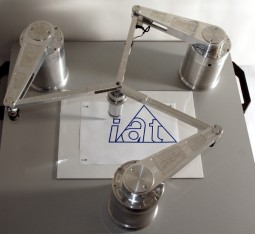
\includegraphics[width=0.6\textwidth]{images/delta2d.png}
    \caption{Imagem acessível em \citeurl{deskriptor2014}}
    \label{fig:my_label}
\end{figure}

\newpage

\printbibliography 

\end{document}
